\documentclass{beamer}
\beamertemplatenavigationsymbolsempty
\usecolortheme{beaver}
\setbeamertemplate{blocks}[rounded=true, shadow=true]
\setbeamertemplate{footline}[page number]
%
\usepackage[utf8]{inputenc}
\usepackage[english,russian]{babel}
\usepackage{amssymb,amsfonts,amsmath,mathtext}
\usepackage{subfig}
\usepackage[all]{xy} % xy package for diagrams
\usepackage{array}
\usepackage{multicol}% many columns in slide
\usepackage{hyperref}% urls
\usepackage{hhline}%tables
\usepackage{graphicx}

% Your figures are here:
\graphicspath{ {fig/} {../fig/} }

%----------------------------------------------------------------------------------------------------------
\title{Поиск границ радужки\\ методом круговых проекций}
\author[А.\,А. Баженов]{Баженов Андрей Александрович}
\institute{Московский физико-технический институт}
\date{\footnotesize
\par\smallskip\emph{Курс:} Автоматизация научных исследований\par (практика, В.\,В.~Стрижов)/Группа 821
\par\smallskip\emph{Эксперт, консультант:} И.\,А.~Матвеев
\par\bigskip\small 2021}
%----------------------------------------------------------------------------------------------------------
\begin{document}
%----------------------------------------------------------------------------------------------------------
\begin{frame}
\thispagestyle{empty}
\maketitle
\end{frame}

\begin{frame}{Поиск границ}
\begin{block}{Цель исследования}
Применение метода круговых проекций яркости для понижения размерности в задаче обработки изображений.
\end{block}
\begin{block}{Задача}
Построить алгоритм нахождения приблизительных границ элементов глаза на чёрно-белых фотографиях. 
\end{block}
\end{frame}

\begin{frame}{Круговые проекции яркости}
\begin{columns}[c]
\column{0.5\textwidth}
		\begin{picture}(100,50)
				\put(0, -10){
	  			\includegraphics[scale=0.3]{img/eye_only.png}}
	 			\put(45, 45){\vector(-4, -1){15}}
	 			\put(25, 30){$\vec{g}(\vec{x})$}
    	\end{picture}

    	\bigskip
    	$\vec{x}$~--- точка изображения\\ 
    	$b(\vec{x})$~--- яркость в точке \\
		$\vec{g}(\vec{x}) = \nabla b(\vec{x})$
	
\column{0.5\textwidth}
		\includegraphics[scale=0.3]{img/projs.png}
	
		$v_U(\vec{x})$~--- индикатор принадлежности границе\\
		$\Pi_U(r)$~--- усредненное значение индикатора по кругу радиуса $r$
\end{columns}
\end{frame}

\begin{frame}{Литература}

\begin{block}{Обзор алгоритмов обнаружения радужки}
	\begin{enumerate}
			\item A.~Nithya and C.~Lakshmi. Iris Recognition Techniques: A Literature Survey. 2015
			\item K.~Bowyer, K.~Hollingsworth, and P.~Flynn. Image Understanding for Iris Biometrics: A Survey. 2008
	\end{enumerate}
\end{block}

\begin{block}{Описание метода круговых проекций}
		\begin{enumerate}
				\item I.\,A.~Matveev. Detection of iris in image by interrelated maxima of brightness gradient projections. 2010
		\end{enumerate}
\end{block}

\end{frame}

\begin{frame}{Задача нахождения границ радужки}

Задана выборка растровых изображений:
\[\mathcal{M} = \left\{\left(M(i), P_\text{R}(i), I_\text{R}(i)\right)\right\}_{i=1}^n.\]

\begin{block}{Требуется построить алгоритм}
\vspace{-0.4cm}
\[
	f\!: \quad M \mapsto \left(P_\text{R}, I_\text{R}\right).
\]
\end{block}

\begin{block}{Рассматриваются модели вида}
\vspace{-0.4cm}
\[
f = \varphi \circ \Pi,
\]
$\Pi$~--- процедура подсчета круговых проекций,
\[
\varphi(t) = \sigma_k\large\left(W_k^T \sigma_{k-1}\large\left(\ldots \sigma_1\left(W_1^T t\right)\ldots\large\right)\large\right).
\] 

\end{block}
\vspace{-0.3cm}
\begin{block}{Задача оптимизации}
\vspace{-0.4cm}
\[
f_0 = \arg\min_{f \in \mathcal{F}} \sum_{i=1}^n L\left(\widehat{P}_\text{R}(i), P_\text{R}(i)\right) + L\left(\widehat{I}_\text{R}(i), I_\text{R}(i)\right).
\]
\end{block}
\end{frame}

\begin{frame}{Обработка круговых проекций}

\begin{block}{Зависимость круговой проекции от радиуса}
\begin{center}
\includegraphics[scale=0.27]{img/projs.png}
\end{center}
\end{block}
\vspace{-0.5cm}
\begin{block}{Гипотеза}

Значения $P_\text{R}$ и $I_\text{R}$ являются точками локальных максимумов функции $\Pi_U(r)$.

\end{block}

\bigskip

Для выделения максимумов и их обработки используются линенйные, сверточные и реккурентные нейронные сети, обучаемые по метрике MSE.

\end{frame}

\begin{frame}{Вычислительный эксперимент}

\begin{block}{Цель}
Сравнить модели по параметрам:
\begin{enumerate}
		\item Точность решения;
		\item Скорость работы.
\end{enumerate}
\end{block}

\begin{block}{Обучаемые модели}
Архитектуры для обработки временных рядов:
\begin{enumerate}
		\item Рекурсивные сети;
		\item Сверточные сети.
\end{enumerate}
Простейшие модели:
\begin{enumerate}
		\item Полносвязная сеть;
		\item Эвристический алгоритм.
\end{enumerate}
\end{block}

\end{frame}

\begin{frame}{Результаты эксперимента}
\begin{block}{Кривые обучения с доверительным интервалом}
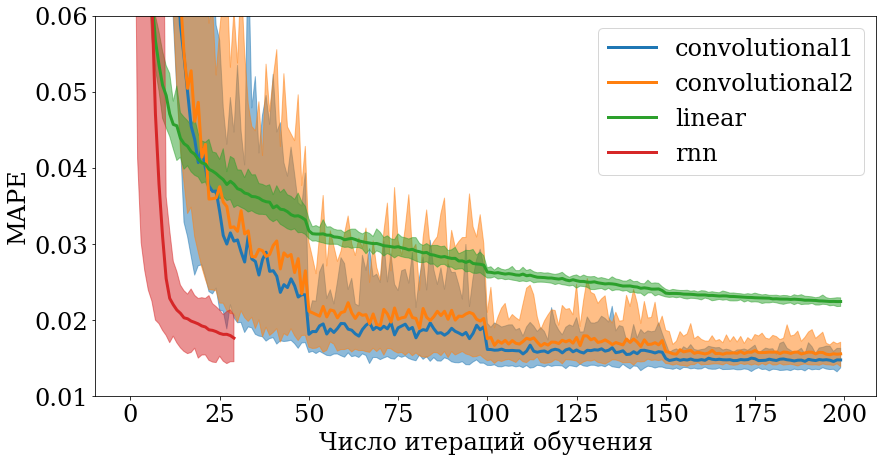
\includegraphics[scale=0.33]{img/mape.png}
\end{block}

\end{frame}

\begin{frame}{Результаты эксперимента}

\begin{center}

\begin{tabular}{|c|m{1.9cm}|m{2.3cm}|m{2.5cm}|}
\hline
Архитектура & Число \mbox{параметров} & Средняя ошибка, \% & Доверительный интервал\tabularnewline
\hline
Полносвязная & $166402$ & $2.21$ & $2.15$-$2.24$\tabularnewline
Сверточная & $56831$\ & $1.39$ & $1.32$-$1.47$\tabularnewline
Сверточная & $17655$ & $1.48$ & $1.39$-$1.58$\tabularnewline
Реккурентная & $14962$ & $1.77$ & $1.45$-$2.05$\tabularnewline
\hline
\end{tabular}
\end{center}
При меньшем числе параметров модели, точность сверточной и реккурентной моделей выше.

\end{frame}

\end{document}